\documentclass[runningheads]{llncs}
\usepackage[ngerman]{babel}
\usepackage{graphicx}
\usepackage{placeins}
\usepackage{hyperref}
\usepackage{amssymb,amsmath, amsthm}

\begin{document}
\title{Bericht: Drohnenverfolgung mit PTZ-Kamera}
\author{Merlin, Vincent, Pablo}
\titlerunning{Bericht: Drohnenverfolgung mit PTZ-Kamera}

\institute{Rheinische Friedrich Wilhelm Universität Bonn }
\date{April 2021}



\maketitle

\begin{abstract}
Es wurde ein Programm entwickelt, welches die automatische Verfolgung einer fliegenden Drohne durch eine PTZ-Netzwerkkamera-Kamera ausführt. Das Programm verfügt über Scan- und Tracking- Modi und prozessiert iterativ aufgenommene Frames in einem Ablauf aus Detektion mit YOlO, Tracking mit Kalman und Kamerasteuerung. Die Funktion des Drohnenverflogungsprogramms wurde in mehreren Testszenarien erfolgreich demonstriert.
\end{abstract}


\section{Motivation}
Mit der steigenden Verbreitung von zivilen Drohnen steigen auch die Möglichkeiten der schädlichen Verwendung. Ein Beispiel für eine solche schädliche Verwendung ist der Gatwick Airport Vorfall 2018, bei dem die Sichtung von Drohnen auf dem Flughafengelände zu einer temporären Einstellung des Flugverkehrs führte. Zivile Drohnen bergen jedoch nicht nur ein wirtschaftliches Gefährdungspotential. Auch in der Kriegsführung können zivile Drohnenmodelle genutzt werden, zur Aufklärung oder zum Abwurf von Sprengladungen.\\\\
Folglich gibt es ein hohes Interesse an wirksamen Systemen zur Erkennung von Drohnen, um ggf nach einer Erkennung Abwehrmaßnahmen einleiten zu können.\\\\
Eine mögliche Methode zur Erkennung von Drohnen ist die optische Detektion mitilfe von Kameras und echtzeitfähigen Deep-Learning-Detektionsmodellen. Im Gegensatz zur Radardetektion ist diese Detektionsmethode passiv, also ohne Emittierung von Strahlung, was insbesondere im militärischem Kontext von Vorteil ist.\\\\ Die Detektionsmodelle müssen schnell predizieren können, um eine Kamerasteuerung in Echzeit zu ermöglichen, und sie müssen zuverlässig und präzise Drohnen detektieren können. Diese Anforderungen sollen durch state-of-the-art-Detektionsmodelle wie YOlOv8 oder RT-DETR erfüllt werden. \\\\
Da die Ergebnisse der Detektionsmodelle fehlerbehaftet sein können, ist für das Verfolgen der Drohnenflugbahn die Verwendung von Trackingalgorithmen von Vorteil. Ein besonders verbreiteter und fundamentaler Trackingalgorithmus ist der Kalman-Filter.

\begin{figure}
    \centering
    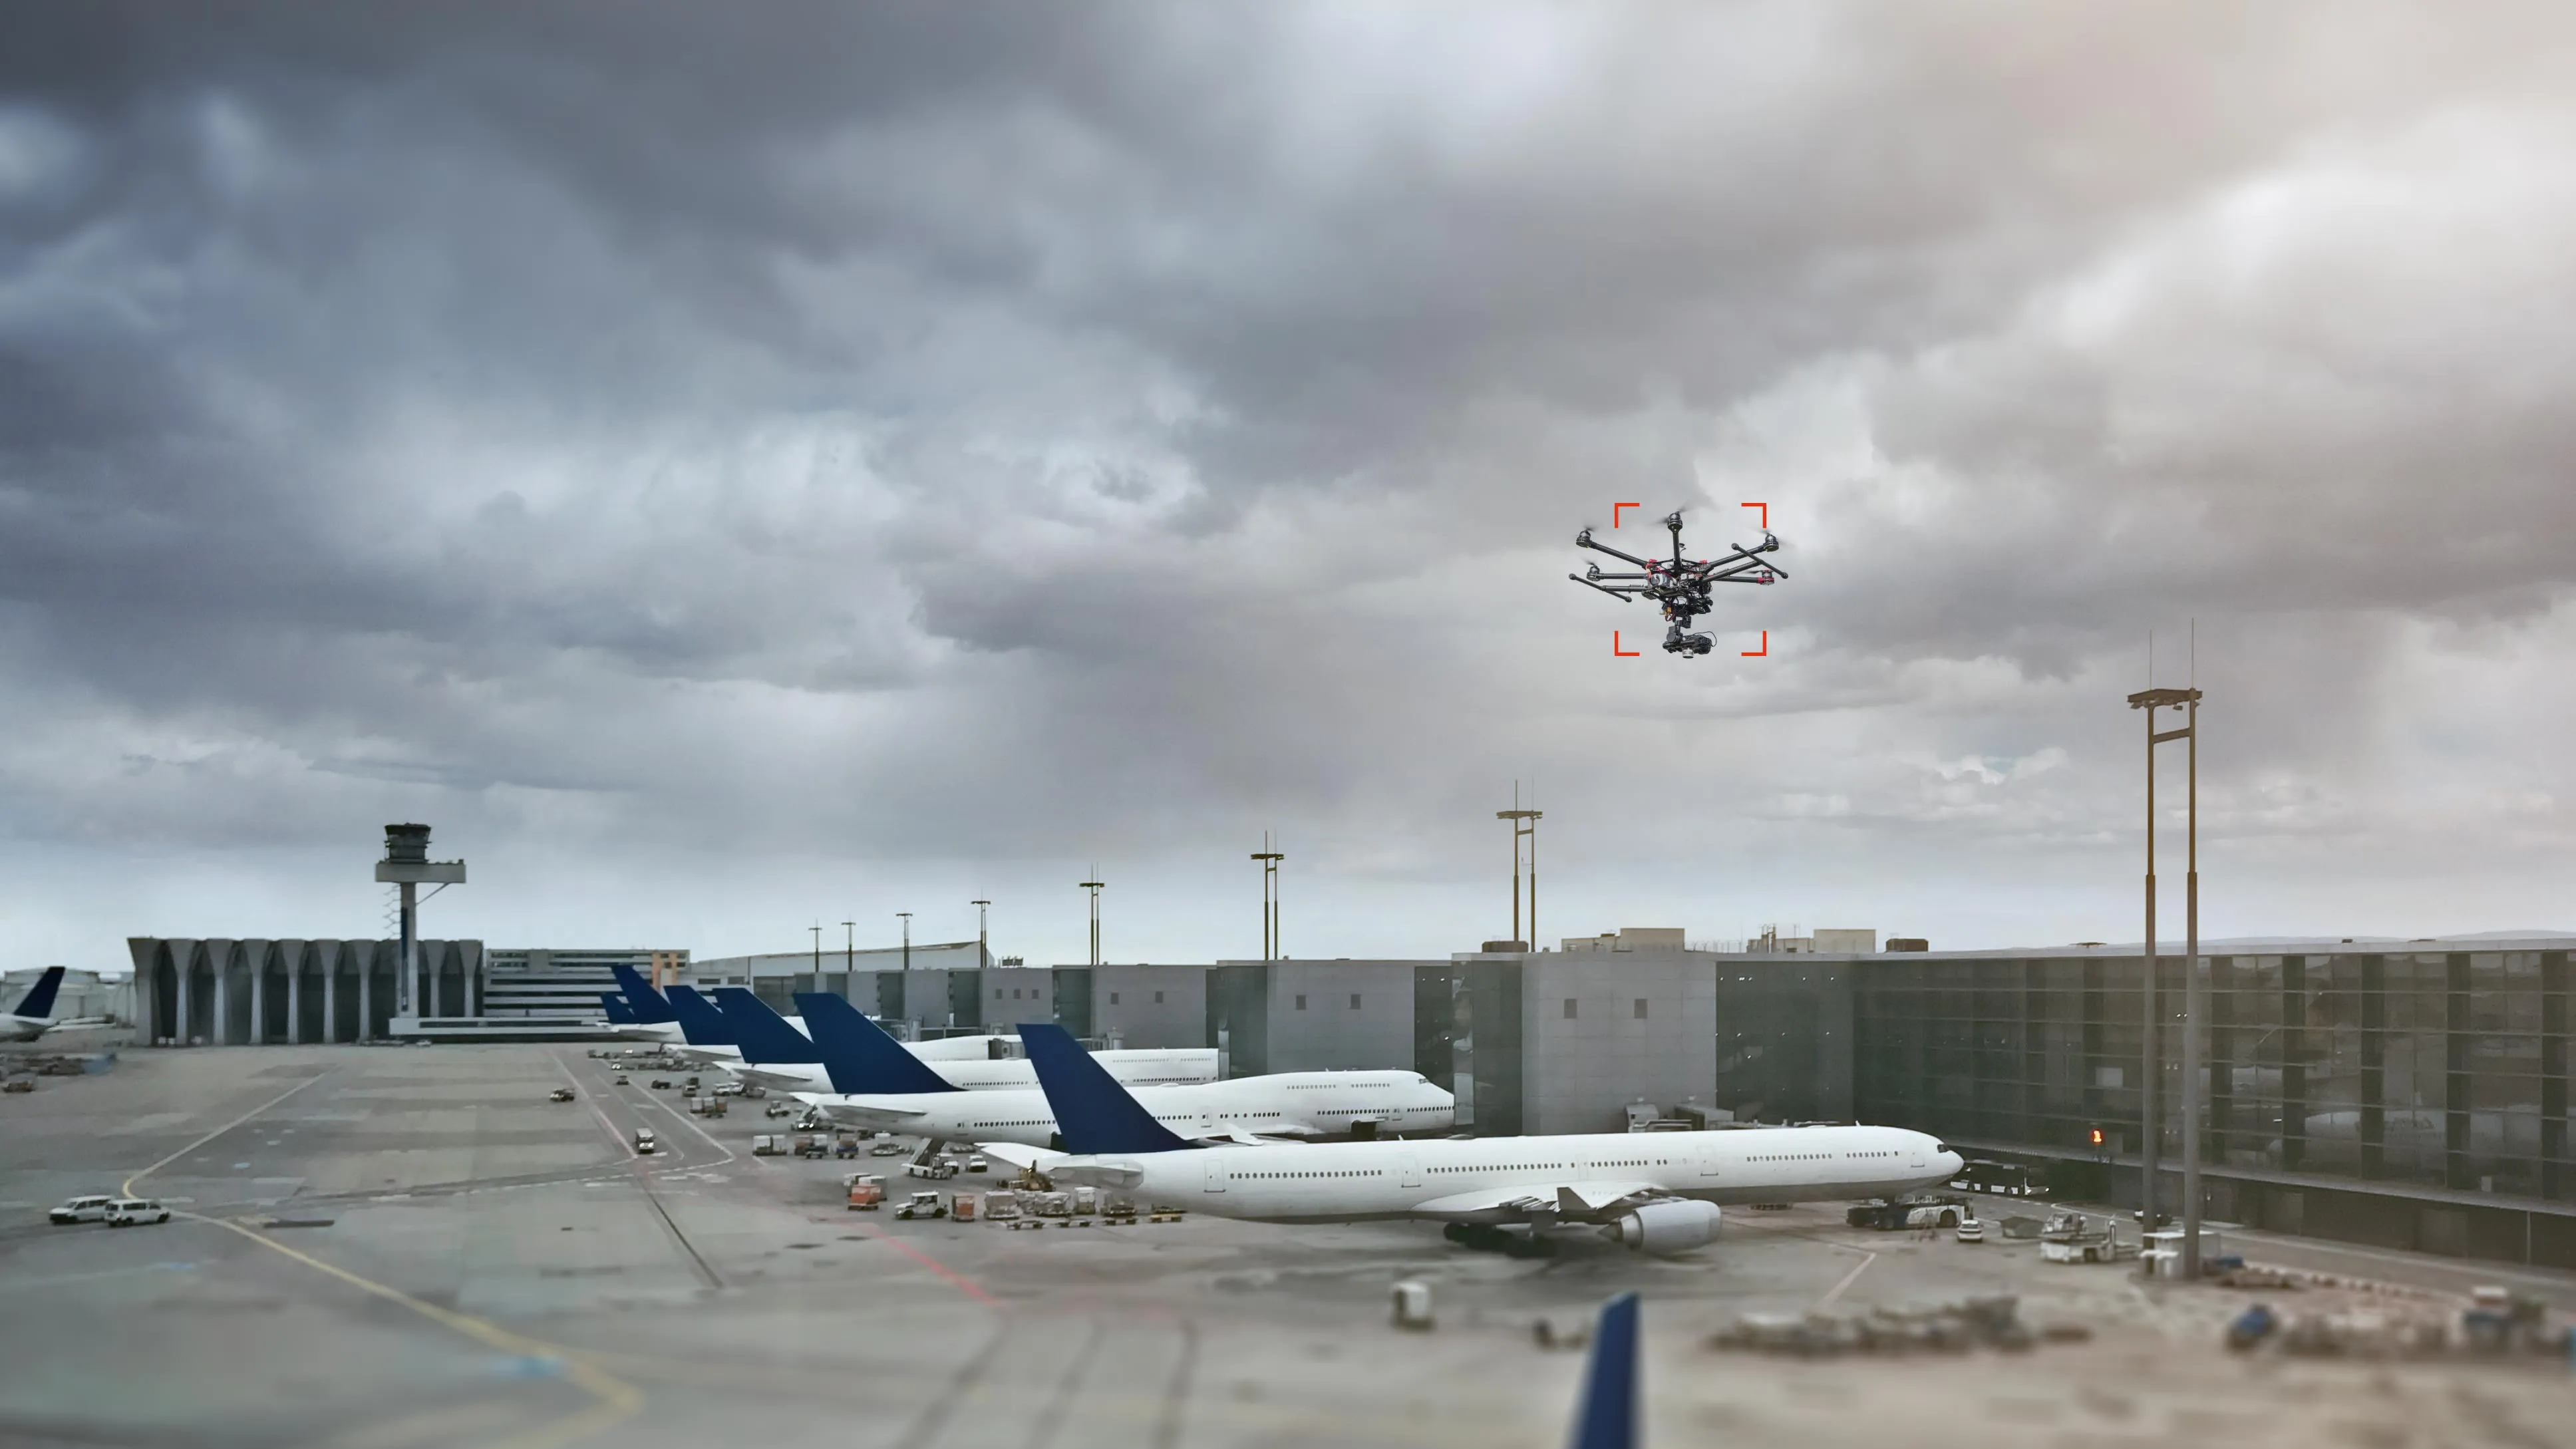
\includegraphics[scale=0.05]{Drohne_flughafen.png}
    \caption{Detektion einer Drohne auf einem Flughafengelände}
\end{figure}
\FloatBarrier

\subsection{Verwandte Arbeiten}

Lassen wir das weg? Spart jedenfalls Arbeit

\section{Theorie}

\subsection{YOLOv8}
YOLO \cite{YOLO} (You Only Look Once) ist ein Objektdetektionsmodell. Es ist ein sog. One-Stage-Detektor. Im Gegensatz zu den ebenso populären Two-Stage-Detektoren wird die Objektdetektion in einem einzigen Vorwärtsdurchlauf durchgeführt und das Netz verzichtet auf eine Vorstufe mit Regionsvorschlägen.\\\\
YOLOv8 unterscheidet sich architektonisch nur gerinfügig von YOLOv5 und bringt im Wesentlichen Vereinfachungen in der Nutzbarkeit für Entwickler und Anwender mit sich. YOLOv5 wiederum ist auch eine architektonische Weiterentwicklung von YOLO.\cite{YOLOv5}\\\\ Das CSPDarknet53-Backbone erweitert das ursprüngliche Darknet-Backbone um die Cross-Stage-Partial-Technik. Diese partioniert Feature Maps und führt die Partitionen in einer späteren Schicht wieder zusammen.\\\\ Der sogenannte Head bildet Feature Maps, die es vom sog. Neck erhält, auf die finalen Prediktionen ab. Der Neck dient als Verbindungsglied zwischen Head und Backbone. YOLOv5 verwendet als Neck ein Spatial-Pyramid-Pooling-Netzwerk (SPP). SPP wendet mehrere Pooling-Operationen mit verschiedenen Rastergrößen auf eine Feature-Map an und kombiniert die Resultate zu ner einzelnen Merkmalsrepräsentation. SPP hat einen positiven Effekt auf die Detektion von Objekten unterschiedlicher Größen. 


\subsection{RT-DETR}

\subsection{Evaluationsmetrik}
Für die Bewertung der Qualität der Prediktionen eines Detektionsmodells bedarf es einer Evaluationsmetrik. Diese beruht auf den bekannten statistischen Größen Präzision und Recall, welche sich aus der Anzahl an true positives, false positives und false negatives berechnen.\\\\
Es muss jedoch erst definiert werden, wann eine Prediktion überhaupt als true positive oder false positive gilt. Dazu wird der IoU-Wert verwendet. Bei diesem handelt es sich um dem Quotienten aus der Schnittmenge und Vereinigung der vorhergesagten und tatsächlichen Bounding Box bzw Maske.\\\\
Nun kann ein Objekt als true positive bzw. false positive eingeteilt werden, wenn der zugehörige IoU-Wert über oder unter einem definierten Schwellwert liegt. Als primäre Metrik wird oft die (irreführend benannte) Average Precision (AP) verwendet. Dabei handelt es sich nicht lediglich um den Mittelwert von Präzisionen nach obiger Formel. Die Präzision alleine genügt nicht als Metrik, da sie von false negatives unbeeinflusst ist. Das genaue Vorgehen zur Berechnung der AP kann sich im Detail unterscheiden. Im Allgemeinen wird jedoch eine Precision-Recall-Kurve bestimmt, welche Präzision und Recall für unterschiedliche Konfidenzwerte der Prediktionen angibt, und  es wird die Fläche unter der Kurve als Maßstab für die Qualität des Modells abgeschätzt.\cite{Metriken} Die primäre COCO--Präzisionsmetrik ist der Mittelwert der APs bei Verwendung von IoU-Schwellwerten von 0.5 bis 0.95 in Schritten von 0.05.\cite{COCO-Metrik}

\subsection{Kalman-Filter}
Der Kalman-Filter ist ein Algorithmus, um aus einer Zeitreihe von fehlerbehafteten Messungen einen durch eine Wahrscheinlichkeitsdichte beschriebenen Zustand abzuschätzen. Der Kalman-Filter folgt direkt aus den fundamentalen Bayesischen-Trackinggleichungen, wenn man die Annahme von normalverteilten Zuständen anlegt. Der Kalman-Filter führt iterativ die Schritte Prediktion und Filterung durch.

\section{Datensatz}
Bei der Sichtung öffentlich verfügbarer Drohnendatensätze wurde kein einzelner Datensatz gefunden, der alleine eine gute Generalisierung ermöglichen würde. Die Datensätze bestanden meist aus Bildern, in denen sich die Drohne stark im Vordergrund befindet und der Hintergrund homogen ist. Ein zu Testzwecken durchgeführtes Training mit einem öffentlich verfügbaren Datensatz führte zu unbefriedigenden Resultaten mit vielen Falschpositivdetektionen.\\\\
Es wurde deshalb ein neuer Datensatz erstellt, indem aus den öffentliche Datensätzen eine ausgwogene Auswahl von Aufnahmen von von Drohnen in verschiedenen Entfernungen, verschiedenen Umgebungen und Posen entnomment entnommen wurde. Weiterhin wurden eigene Bilder in unserem Büro aufgenommen, da Innenaufnahmen in dem Datensatz stark unterrepräsentiert waren. Der Datensatz wurde nach einigen Tests weiter verbessert. Zum Beispiel wurden Bilder von Objekten hinzugefügt, die oft falsch als Drohne klassifiziert wurden, wie z.B. Türklinken und Kabelgewirre. Dies resultierte letztendlich in einen Datensatz aus XXXXX Bildern, welcher nun auch öffentlich (inklusive Annotationen) zur Verfügung gestellt ist. Der Datensatz wurde mit dem Annotationstool "Anylabeling" annotiert. Der gesamte Datensatz wurde klassisch im Verhältnis 80:10:10 in Training-, Validierung- und Testdatensatz unterteilt.

\section{Methodik}
\subsection{Detektionsmodelle}
Es wurde die Bibliothek Ultraytics verwendet, um YOLOv8 und RT-DETR zu trainieren und zu nutzen. Für beide Netze wurde ein Transfer Learning durchgeführt: Es wurde mit öffentlich verfügbaren Gewichte der auf COCO vortrainierten Netze gestartet und diese dann neu auf unserem Drohnendatensatz trainiert. Die Standardwerte der Hyperparameter wurden nicht verändert. Das Training dauerte XXXX Epochen. Für das Drohnenverfolgungsprogramm wurden die Gewichte jener Epoche gewählt, bei denen YOLO bzw. RT-DETR die höchste Präzision auf dem Validierungsdatensatz zeigten.\\\\

Abbildung XXXX zeigt den Verlauf der primären Präzisionsmetrik mAP auf dem Validierungsdatensatz in Abhängigkeit von der Epochenzahl.

Auf dem Testdatensatz wurde mit YOLOv8 bzw. RT-DETR eine Präzision von XXXX bzw XXXX. erzielt. Dabei wurden die Gewichte der Modelle wie oben geschildert gewählt.

\subsection{Tracking}

XXXXHier sollte man sagen, dass wir den Standard-Kalman Filter benutzen und dafür alle Boxen bis auf jene mit der höchsten Wahrscheinlichkeit aussschließen. Vielleicht auch konkreter, wie die Matrizen im Kalman-Filter gewählt sind XXXXXXX

\subsection{Programmaufbau}

Der Quellcode des Programms kann öffentlich heruntergeladen werden XXXXX.\\\\

Ein grober Überblick des Programmablaufs ist durch das Aktivitätsdiagramm in Abbildung XXXX dargestellt. Das Programm kann gedanklich in zwei Modi unterteilt werden; einen Scanmodus und einen Trackingmodus.\\\\ Das Programm startet im Scanmodus. In diesem bewegt dreht sich die Kamera bei minimaler Zoomstufe horizontal um sich selber, mit alternierender Aufwärts- und Abwärtsbewegung. Diese Bewegung dient dazu, regelmäßig unterschiedliche Bereiche des Kamersichtfelds zu erfassen. Im Scanmodus wird iterativ ein Kamerabild aufgenommen und für die Prediktion an das Detektionsmodell YOLO (bzw. RT-DETR, je nach Konfiguration) übergeben. Erst wenn in einem Bild eine Drohnendetektion auftritt, wird der Scanmodus verlassen und in den Trackingmodus übergegangen. Dabei wird der Kalman-Filter des Trackingmoduls (re)-initialisiert.\\\\
Auch im Trackingmodus wird iterativ ein Bild aufgenommen und auf diesem mit dem Detektionsmodell prediziert. Die Detektionsergebnisse werden dann jedoch vom Kalman-Filter verwendet, um die tatsächliche Position der Drohne (in Bildkoordinaten ) abzuschätzen. Anschließend werden die Tracking-Ergebnisse verwendet, um die Drohne zu steuern. Die Kameraausrichtung wird verändert, sodass sich ihr Bildmittelpunkt in Richtung des Trackingergebnisses bewegt. Als zusätzliches Feature wurde implementiert, dass die Kamera abhängig von der Boxgröße der Detektion ihre Zoomstufe vergrößert oder verkleinert. Der Trackingmodus wird verlassen, wenn das Ziel verloren ist. Das Ziel gilt als verloren, wenn in einem konfiguierbaren Zeitraum keine Detektion mehr erfolgte.\\\\

Ungewöhnlich mag erscheinen, dass im Fall einer Nicht-Detektion ohne Zielverlust auf das Verwenden des Trackingalgorithmus und anschließendes Adjustieren der Kamerabewegung verzichtet wird. Der Grund dafür ist, dass die Kamerasteuerung über einen continous-move-Befehl erfolgt (siehe Kapitel Kamerasteuerung). Im Tracking-Modus bewegt sich die Kamera bei Nicht-Detektion ohne Zielverlust also weiterhin in die gleiche Richtung wie in der letzten Iteration mit Detektion. Letztendlich stellt dies also keinen Unterschied dar zur alternativen Vorgehensweise, bei Nichtdetektion das Ergebnis der Kalman-Prediktion für die Kamerasteuerung zu verwenden.


\begin{figure}
    \centering
    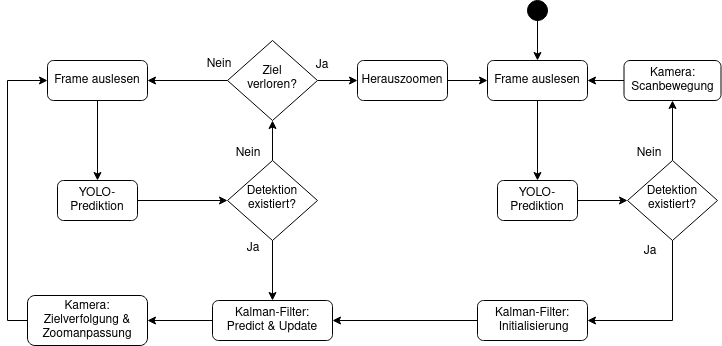
\includegraphics[scale=0.5]{Flussdiagramm.png}
    \caption{Aktivitätsdiagramm des Programmablaufs}
\end{figure}
\FloatBarrier

\subsection{Kamerasteuerung}

Im Allgemeinen erfolgt die Steuerung der Kamera und das Erhalten von Informationen von der Kamera durch das Senden von HTTP-Requests an die IP-Adresse der Kamera. Die genauen URLs der HTTP-Requests wurden der VAPIX-Network-Video-API entnommen.\\\\

Die Steuerung der Kamerausrichtung erfolgt in unserem Drohnenprogramm nicht durch explizite Angabe von absoluten Pan- und Tilt-Werten, sondern durch die Verwendung eines continous-move-requests. Dabei handelt es sich um einen Geschwindigkeitsvektor der Pan- und- Tilt-Bewegung, der an die Kamera übergeben wird. Der Geschwindigkeitsvektor wird so gewählt, dass seine Richtung zur Bildkoordinate des Trackingergebnisses zeigt. Die Größe des Geschwindigkeitsvektors wird proportional zur Differenz der Koordinaten von Bildmittelpunkt und Trackingergebnis gewählt.\\\\

XXXXXX Hier Vorteile und Nachteile davon nennen? Latenz macht bei hohen Geschwinigkeiten Probleme etcXXXXX

\section{Tests und Untersuchungen}

Hier viele Bilder zeigen

\section{Evaluation/Diskussion}
\subsection{Qualität der Detektion}
Die Erzeugung eines qualitativ hochwertigen Datensatzes und das Verwenden von mächtigen Detektionsmodellen ermöglichte die zuverlässige Detektion der Drohne in unserer Testumgebung Büroraum.\\\\
Dennoch waren gelegentlich Falschpositivdetektionen zu beobachten, z.B. von Kabelgewirr oder Zeichnungen auf einem Whiteboard. Dies liegt vermutlich an ähnlichen geometrischen Strukturen, die manchmal gut zu einer Drohne passen. Dieses Problem ließe sich beheben, indem man dem Datensatz mehr Bilder mit drohnenähnlichen Objekten, die keine Drohnen sind, zuführt.\\\\
Da als Testumgebung nur Innenräume zur Verfügung standen, konnte die Performanz der Detektion von weit enfernten Drohnen nicht überprüft werden.\\\\
Leichte Unterschiede durch die Wahl des Detektionsmodells sind beobachtbar: RT-DETR detektiert zuverlässiger und mit höheren Konfidenzwerten als YOLO, jedoch auch deutlich langsamer als YOLO. XXXXXXXXXXX Hier Zahlen nennen, irgendwo sollten wir auch unsere Hardware Specs nennen XXXXXXXXXXXXX
Die langsamere Prediktion von RT-DETR gegenüber YOLO wirkt sich negativ auf die Drohnenverfolgung aus, da es dann eine höherere Latenz zwischen Bildaufnahme und Kamerasteuerung gibt.
Für die Wahl des Detektionsmodells muss man also eine Tradeoff zwischen Detektionsqualität und Latenz abwägen.
\subsection{Qualität der Drohnenverfolgung}
Mit beiden Netzen kann unsere Drohne in unserer Testumgebung zuverlässig mithilfe des Scanmodus gefunden und anschließend verfolgt werden.
Lediglich bei zu hohen Winkelgeschwindigkeiten oder vor einer starken Lichtquelle wird die Drohne öfters verloren.

XXXXXXXXX Ein paar Worte zu Drohnenverfolgung unterschiedliche Zoomstufen XXXXXXX
XXXXXXXXX Ein paar Worte zur Methode der Kamerasteurung? XXXXXXX
\section{Fazit}

\begin{thebibliography}{3}

\bibitem{Flughafenbild}
URL \url{https://www.dedrone.com/industry/airports}, Abrufdatum: 7.9.2023
\bibitem{YOLO}
Girshick, Ross and Donahue, Jeff and Darrell, Trevor and Malik, Jitendra: \textit{You Only Look Once: Unified, Real-Time Object Detection} 
 - URL \url{https://arxiv.org/abs/1506.02640}
 Abrufdatum: 7.9.2023
\bibitem{YOLOv5}
 - URL \url{ https://docs.ultralytics.com/yolov5/tutorials/architecture_description/#1-model-structure}
 Abrufdatum: 7.9.2023
 \bibitem{Metriken}
URL \url{https://github.com/rafaelpadilla/Object-Detection-Metrics}
Abrufdatum: 7.9.2023
 \bibitem{COCO-Metrik}
 URL \url{https://cocodataset.org/\#detection-eval}
 Abrufdatum: 7.9.2023

\end{thebibliography}


\end{document}
